\section{Colore}\label{sec:colore}
\subsection{Definizione di colore}
L'\emph{indice di colore} è la differenza tra le magnitudini misurate in due diverse bande fotometriche (\emph{filtri}). In particolare, le immagini vengono acquisite attraverso filtri che selezionano solamente alcune lunghezze d'onda. Ciascun filtro ha la propria curva di trasmissione, centrata su una data lunghezza d'onda. D'altra parte, ciascuna sorgente ha il proprio spettro di emissione. Quindi, i diversi filtri selezionano solo una frazione dello spettro della sorgente, quella inclusa sotto la loro curva di trasmissione (fig.~\ref{fig:filtri-fotometrici}). Ne conviene che il flusso misurato durante l'osservazione in un dato filtro dipende sia dal filtro che dallo spettro della sorgente.

\begin{figure}
\centering
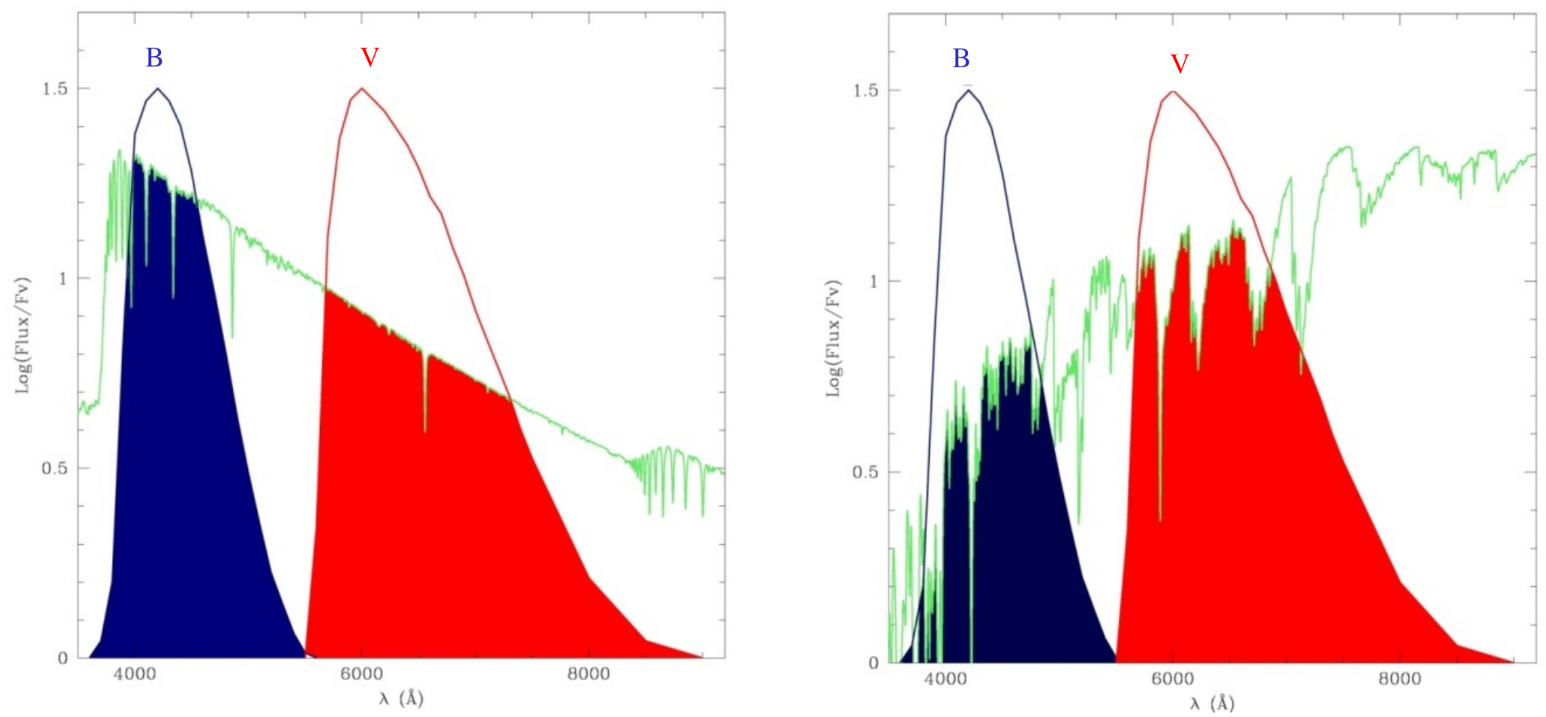
\includegraphics[width=0.7\textwidth]{immagini/filtri-fotometrici.png}
\caption{Osservazione di due spettri diversi con due filtri, uno blu (B) e uno rosso (R). In verde sono rappresentati gli spettri analizzati e le curve in blu e rosso sono rispettivamente le curve di trasmissione del filtro blu e rosso. Le zone evidenziate rappresentano il flusso misurato. Si nota che a sinistra vale $F_B > F_V$ mentre a destra $F_B < F_V$. Ciò evidenzia come il flusso misurato dipende sia dallo spettro della sorgente che dal filtro utilizzato.}
\label{fig:filtri-fotometrici}
\end{figure}

Ricordando l'equazione~\eqref{eq:relazione-magnitudine-apparente-flusso}, si può scrivere:
\[
    m_B = -2.5 \log F_B + \textup{const}
\]
\[
    m_V = -2.5 \log F_V + \textup{const}
\]
dove $m_B$ e $m_V$ sono le magnitudini apparenti rispettivamente in filtro blu e filtro rosso (analogo per i flussi misurati $F_B$ e $F_V$). Si definisce \emph{colore} la differenza tra la magnitudine misurata col filtro più blu e la magnitudine misurata col filtro più rosso:
\begin{equation}\label{eq:colore}
    m_B - m_V \equiv B-V
\end{equation}
Il colore, dunque, è un numero puro, e in tab.~\ref{tab:colore} sono presenti le relazioni tra il colore, la magnitudine assoluta e il flusso in filtro blu e rosso. 

\begin{table}
\caption{Relazione tra colore, magnitudine apparente e flusso.}
\label{tab:colore}
\centering
\begin{tabular}{lll}
\toprule
Colore & Magnitudine apparente & Flusso \\
\midrule
$<0$ & $m_B < m_V$ & $F_B > F_V$ \\
$=0$ & $m_B = m_V$ & $F_B = F_V$ \\
$>0$ & $m_B > m_V$ & $F_B < F_V$ \\
\bottomrule
\end{tabular}
\end{table}

Ovviamente, cambiamo i filtri, cambia anche la denominazione del colore. Si tenga inoltre in considerazione che il colore \emph{non} dipende dalla distanza, poiché usando le equazioni~\eqref{eq:relazione-magnitudine-apparente-flusso} e~\eqref{eq:flusso} si ottiene che la differenza tra le magnitudini apparenti e le magnitudini assolute è uguale:
\begin{equation}\label{eq:differenza-magnitudini-apparente-assoluta}
    m_B-m_V = M_B-M_V
\end{equation}

\subsection{Colore e temperatura}
Ci si può chiedere quale sia la ragione fisica alla base del diverso colore delle stelle. Ripensando all'esempio in fig.~\ref{fig:filtri-fotometrici} è evidente che una stella è tanto più blu quanto maggiore è il flusso misurato a basse lunghezze d'onda. Dunque, in definitiva, la ragione fisica del diverso colore è la stessa del diverso spettro. Come introdotto nel par.~\ref{sec:legge-planck} ed evidenziato in fig.~\ref{fig:stelle-corpi-neri}, le stelle in prima approssimazione sono dei corpi neri, dunque lo spettro è definito dall'equazione di Planck~\eqref{eq:corpo-nero}. Utilizzando un particolare filtro, si sta fissando la lunghezza d'onda (o frequenza) di picco a cuiˆ'0987 5        c v
     bhcv lavora tale filtro, dunque lo spettro osservato di una stella dipenderà solamente dalla sua \emph{temperatura superficiale}. Ricordando la relazione tra intensità e luminosità monocromatica~\eqref{eq:luminosità-monocromatica-intensità} e imponendo per una stella $I_\nu = B_\nu (T)$ si ottiene:
\[
    L_\nu = 4 \pi R^2 \pi B_\nu (T)
\]
da cui, attraverso la relazione~\eqref{eq:magnitudine-assoluta-luminosità}, usando~\eqref{eq:differenza-magnitudini-apparente-assoluta}, si ottiene
\[
    m_{\lambda 1} - m_{\lambda 2} = M_{\lambda 1} - M_{\lambda 2} = -2.5 \log\frac{L_{\lambda 1}}{L_{\lambda 2}} + \textup{const} = -2.5 \log\frac{B_{\lambda 1}(T)}{B_{\lambda 2}(T)} + \textup{const}
\]
da cui si può inferire che, nel limite di validità dell'approssimazione della stella come corpo nero, il colore dipende solamente dalla temperatura.

Per riassumere, più bassa è la temperatura superficiale, più rossa è la stella, che equivale a un grande $(B-V)$, mentre più alta è la temperatura superficiale, maggiore è il flusso a basse $\lambda$ (cfr. fig.~\ref{fig:corpo-nero}) e più blu è la stella, che equivale a un piccolo $(B-V)$.

\subsection{Estinzione}\label{sec:reddening}
In generale, a causa dei processi d'interazione tra radiazione e materia nel cammino tra la sorgente e l'osservatore, una stella tende ad apparire \emph{più debole} e \emph{più rossa} di come non sia veramente, questo fenomeno prende il nome di \emph{estinzione} (o arrossamento). È possibile esprimere tale fenomeno analiticamente, introducendo un parametro di correzione alla magnitudine "intrinseca", ovvero quella che vedremmo se non ci fosse l'interazione con il mezzo interstellare.
\begin{equation}\label{eq:estinzione}
    m_\lambda = m_{\lambda 0} + A_\lambda
\end{equation}
dove $m_\lambda$ è la magnitudine osservata, $m_{\lambda 0}$ quella intrinseca e $A_\lambda$ prende il nome di \emph{parametro di estinzione}. Esso è relativo alla direzione in cui viene osservata la stella e dipende fortemente dalla lunghezza d'onda, in particolare $A_\lambda$ cresce al diminuire di $\lambda$. La dipendenza di $A_\lambda$ da $\lambda$, detta \emph{legge di estinzione}, è tuttavia scarsamente nota: dipende infatti dalle proprietà del mezzo interstellare lungo la linea di vista, quindi sicuramente cambia al variare della linea di vista, e cambia al variare della galassia che si sta considerando.

È presente una legge di estinzione standard per la Via Lattea, derivata da \emph{Cardelli} (1989), tuttavia probabilmente non è valida ovunque nella nostra galassie e non è chiaro se debba valere anche per altre galassie. L'unica cosa chiara è che l'effetto dell'estinzione cresce al diminuire delle lunghezze d'onda.

Per spiegare l'effetto del \emph{reddening} consideriamo due filtri particolari, un B e un V, e utilizziamo l'equazione~\eqref{eq:estinzione} in combinazione con la~\eqref{eq:colore}. Possiamo scrivere:
\[
    m_\lambda - m_{\lambda 0} = A_\lambda
\]
\[
    B - B_0 = A_B \qquad V - V_0 = A_V
\]
e sottraendo membro a membro:
\[
    B_0 - V_0 \equiv (B-V)_0 = (B-V) - (A_B - A_V)
\]
Il primo termine, $(B-V)_0$, rappresenta il \emph{colore intrinseco}, $(B-V)$ rappresenta il \emph{colore osservato}, mentre l'ultimo termine, $(A_B-A_V) \equiv \EBV$ rappresenta il \emph{reddening}, ovvero l'eccesso di colore. Partendo dal reddening dei filtri B-V si può indicare l'effetto per dei filtri qualunque, moltiplicando per un opportuno fattore correttivo $R_\lambda$:
\begin{equation}\label{eq:reddening}
    m_\lambda = m_{\lambda 0} + A_\lambda = m_{\lambda 0} + R_\lambda \EBV
\end{equation}

\subsection{Modulo di distanza e reddening}
Si faccia attenzione al fatto che la magnitudine apparente che compare nell'espressione del modulo di distanza~\eqref{eq:modulo-distanza} è quella \emph{vera}, ovvero de--arrossata. Talvolta, tuttavia, in letteratura si trova il modulo di distanza \emph{osservato}, ad esempio, in banda V. In questo caso, per trovare la distanza, è necessario de--arrossare:
\[
    (m - M)_V = -5 + 5 \log(d_{\si{pc}}) + 3.12 \, \EBV
\]
Si faccia attenzione anche a un'ultima cosa: la magnitudine assoluta, per definizione, è sempre quella vera. Non ha senso parlare di magnitudine assoluta arrossata.